\chapter{\IfLanguageName{dutch}{Stand van zaken}{State of the art}}%
\label{ch:stand-van-zaken}

% Tip: Begin elk hoofdstuk met een paragraaf inleiding die beschrijft hoe
% dit hoofdstuk past binnen het geheel van de bachelorproef. Geef in het
% bijzonder aan wat de link is met het vorige en volgende hoofdstuk.

% Pas na deze inleidende paragraaf komt de eerste sectiehoofding.
\section{Definities}

\begin{itemize}
    \item \textit{Container: Een container is een standaard software-eenheid die code en al zijn afhankelijkheden verpakt, zodat de toepassing snel en betrouwbaar van de ene computeromgeving naar de andere draait \autocite{Docker-2023}. Containers zijn lichtgewicht en bevatten alles wat nodig is om de applicatie te draaien, dus u hoeft niet te vertrouwen op wat er momenteel op de host is geïnstalleerd. \autocite{DockerDocs-2023} }
    \item \textit{Docker: Docker biedt de mogelijkheid om een aplicatie te verpakken en uit te voeren in een geïsoleerde omgeving, genaamd een container.  \autocite{DockerDocs-2023} }
\end{itemize}

\ref{fig:KubernetesContainers} Geeft een beter beeld wat containers zijn en welke functie docker heeft.

\begin{flushleft}
    \begin{figure}[h]
        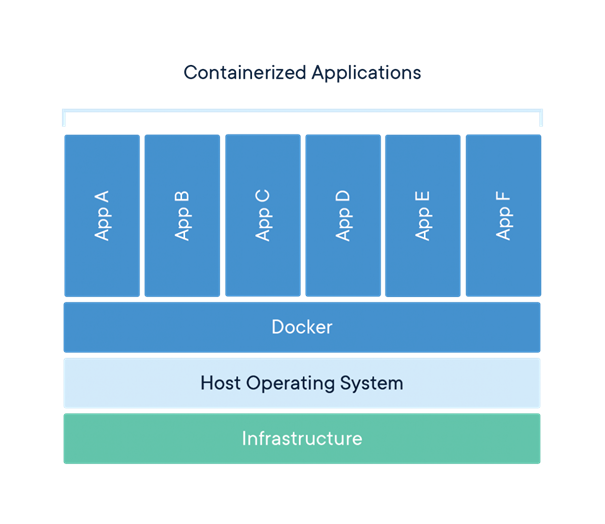
\includegraphics[width=.49\textwidth]{graphics/container.png}
        \caption{\label{fig:KubernetesContainers}Container architectuur \autocite{Docker-2023}}
    \end{figure} 
\end{flushleft}

\section{Kubernetes}
Kubernetes, ook wel afgekort als K8s, is een gratis en open-source systeem dat wordt gebruikt om de implementatie, schaling en het beheer van containerapplicaties te automatiseren. 
Het biedt de mogelijkheid om containers die deel uitmaken van een applicatie te groeperen en te beheren als logische eenheden, waardoor het gemakkelijk wordt om deze te ontdekken en te beheren \autocite{KubernetesDocs-2023}.
Docker is een containerisatieplatform, terwijl Kubernetes een orkestratietool is voor het beheer van meerdere containers.
Docker biedt een eenvoudige en efficiënte methode voor het aanmaken en inzetten van containers, terwijl Kubernetes complexere functionaliteit biedt voor het beheer van containers op schaal \autocite{banerjee-2023}.
Voor grotere, complexere projecten die uitgebreid containerbeheer vereisen, is Kubernetes een krachtiger en flexibeler hulpmiddel.

\subsection{Componenten}
\autocite{KubernetesDocs-2023} Bij het ontplooien van kubernetes ontstaat er een cluster. Een cluster bestaat uit een groep machines zogenaamd "worker nodes". Zo een node heeft verschillende componenten zoals een Kubelet, een kube-proxy en een container-runtime.
Binnen deze worker nodes zijn er pods met containers in. In deze containers kunnen applicaties zoals een SQL database of een website draaien. 
\autocite{KubernetesDocs-2023} Binnen een cluster is er ook een control plane die de globale beslissingen neemt over bijvoorbeeld scheduling of een pod starten. De control plane beheert ook de nodes. 
\autocite{KubernetesDocs-2023} Een control plane bestaat uit verschillende componenten zoals een Kube-apiserver, etcd, kube-scheduler en een kube-controller-manager.
Om voor fouttolerantie en hoge beschikbaarheid te zorgen, draait de control plane in productiescenario's meestal op vele machines, en een cluster bevat doorgaans meerdere nodes \autocite{KubernetesDocs-2023}. 
In leer- of middelenbeperkte omgevingen is er meestal maar één node aanwezig.

Hieronder volgt een lijst met belangrijke terminologie binnen Kubernetes:

\begin{itemize}
    \item Een pod is een groep van één of meer containers \autocite{habbal-2020}. Alle containers in een pod delen hetzelfde IP adres en dezelfde middelen zoals volumes \textcite{hohn-2020}. In makkelijkere woorden is een pod een enkele instantie van een applicatie die kan worden gerepliceerd als er meer instanties nodig zijn om de toenemende druk op te vangen \textcite{habbal-2020}. Gerepliceerde pods zijn creeert en beheert als een groep door de middelen en de control plane \textcite{kubernetesDocs-2022}. 
    \item \textit{Een service is een methode om een netwerktoepassing die als een of meer Pods in uw cluster draait, bloot te stellen \autocite{kubernetesDocs-2022}.} 
\end{itemize}
 









\textcite{Knuth1998} schreef een van de standaardwerken over sorteer- en zoekalgoritmen. Experten zijn het erover eens dat cloud computing een interessante opportuniteit vormen, zowel voor gebruikers als voor dienstverleners op vlak van informatietechnologie~\autocite{Creeger2009}.

\lipsum[7-20]

